\documentclass[10pt,a4paper]{article}
\usepackage[utf8]{inputenc}
\usepackage[british]{babel}


\usepackage{amsmath, amsfonts, amssymb, array, amsthm}
\usepackage[tmargin=1in,bmargin=1in,lmargin=1.25in,rmargin=1.25in]{geometry}
\usepackage{sectsty} % control section /header style
\usepackage{fancyhdr}
\usepackage{hyperref} 
\usepackage{mathtools} %for prescript function in permutation command
\usepackage{cancel} %gives \cancel command
\usepackage{gensymb} %for the \degree command
\setlength{\jot}{5mm} %Line Spacing in the gather environment

\usepackage{xcolor}
% Define colours
\definecolor{blu2}{HTML}{206B99}
\definecolor{plumb}{HTML}{A16E83}
\definecolor{pink1}{HTML}{E18AAA}
\definecolor{pink2}{HTML}{DA7B93}
\definecolor{gren}{HTML}{B4D3B2}
%%%%%%%%%%
\definecolor{blu1}{HTML}{5DA2D5}
\definecolor{lightblu}{HTML}{90CCF4}
\definecolor{red1}{HTML}{F78888} %#ecb4b4
\definecolor{red2}{HTML}{EDB5BF}
\definecolor{lilacc}{HTML}{86B3D1}
\definecolor{gren1}{HTML}{b4ecb4}
\definecolor{gren2}{HTML}{73dc73}
%%%%%%%%%%
\definecolor{navi}{HTML}{4E576E}
\definecolor{blumb}{HTML}{71475B}
%%%%%%%%%%
\hypersetup{colorlinks=true, linkcolor=blumb, urlcolor=blumb, filecolor=blu2, citecolor=blumb}

% Title and Subtitle
\newcommand{\Title}[1]{\begin{center}\textcolor{navi}{\begin{Huge}#1\vspace{1pt}\end{Huge}}\end{center}}
\newcommand{\SubTitle}[1]{\begin{center}\textcolor{navi}{#1\vspace{1pt}}\end{center}}
\newcommand{\NB}[1]{\textcolor{blumb}{\textbf{NB: }}}
% Other Commands
%\newcommand\Perm[2][^n]{\prescript{#1\mkern-2.5mu}{}P_{#2}}
%\newcommand\Comb[2][^n]{\prescript{#1\mkern-0.5mu}{}C_{#2}}

\newcommand*{\Perm}[2]{{}^{#1}\!P_{#2}}
\newcommand*{\Comb}[2]{{}^{#1}C_{#2}}

% Color of Headings
\subsectionfont{\color{navi}}
\sectionfont{\color{blumb}}
\subsubsectionfont{\color{blumb}} 

\begin{document}

\Title{L.C. Physics Derivations}
\SubTitle{Oisín Peppard}
\SubTitle{June 2022}
\hrulefill

There are very few derivations on the leaving cert physics syllabus. They're probably the easiest way to pick up guaranteed marks, the next easiest being definitions and specified demonstrations.

\section{Mechanics}

\subsection{Linear Motion}
We must derive the three equations of linear motion, where the symbols have their usual meanings. The first is simple, just rearrange the definition of acceleration as average change in velocity over time.

\begin{align*}
    a &= \cfrac{v-u}{t} \\
    v &= u + at 
    \quad \qedsymbol
\end{align*}

We then have the second equation. Which comes from declaring displacement equal to average velocity $\times$ time.

\begin{gather*}
    s = (\cfrac{u + v}{2}) \cdot t \\
    = \cfrac{u + (u + at)}{2} \cdot t \\
    = ut + \cfrac{1}{2} \cdot at^2
    \quad \qedsymbol
\end{gather*} 
And finally the third, which begins by squaring the result of the first.

\begin{gather*}
    v^2 = (u + at)^2 \\
    v^2 = u^2 + 2uat + (at)^2 \\
    v^2 = u^2 + 2a(ut + \cfrac{1}{2}at^2) \\
    v^2 = u^2 +2as
    \quad \qedsymbol
\end{gather*}

\newpage
\subsection{Newtonian mechanics}
The next derivation in mechanics is to show how Newton's second law - \textbf{(rate of change of momentum $\propto$ impressed force)} - implies a relationship between force and acceleration.

\begin{gather*}
    F \propto \cfrac{dp}{dt} \\
    F \propto \cfrac{d(mv)}{dt} \\
    F \propto m \cfrac{dv}{dt} \\
    F \propto ma \rightarrow F = kma.
\end{gather*}
In SI units we define  \textbf{1 Newton} as the product of \textbf{$\textbf{1kg}$} and $\mathbf{1ms^{-2}}$, and as such $k=1$, leaving us with
\begin{equation*}
    F=ma \quad \qedsymbol
\end{equation*}

\subsection{Circular and Orbital motion}
First we have the relationship between the radius, linear and angular velocities of a body in circular motion. This is done by simply plugging in their definitions of displacement/arc-length over time, and angle over time

\begin{gather*}
    v = \cfrac{l}{t}, \ \omega = \cfrac{\theta}{t} \text{ and } l = r \theta \\ 
    v = \cfrac{r \theta}{t} \\
    v = r\omega \quad \qedsymbol
\end{gather*}

We also have to determine the relationship between period and radius of a satellite in orbit. We do this by equating \textit{centripetal} force with \textit{gravitational} force
\begin{gather*}
    \cfrac{GM\cancel{m}}{r^2} = \cancel{m}r\omega ^2 \text{ and } T = \cfrac{2\pi}{\omega}\\
    \cfrac{GM}{r^2} =  r (\cfrac{2\pi}{T})^2 \\
    T^2 = 4\pi^2 r\cdot \cfrac{r^2}{GM} \\
    T^2 = \cfrac{4\pi^2r^3}{GM} \quad \qedsymbol
\end{gather*}

\subsection{Simple Harmonic Motion}
To show that an object obeying Hooke's law will also execute simple harmonic motion.
\begin{align*}
    F=-ks \\
    ma = -ks \\
    a = -\cfrac{k}{m}s \\
\end{align*}
and if we let $\omega^2 = \cfrac{k}{m}$ then we arrive at the condition for SHM
\begin{equation*}
    a=-\omega^2 s
\end{equation*}

\section{Waves, Sound and Light}
The only one here is to derive the diffraction grating formula, which is done entirely with a diagram

\begin{figure}[h]
    \centering
    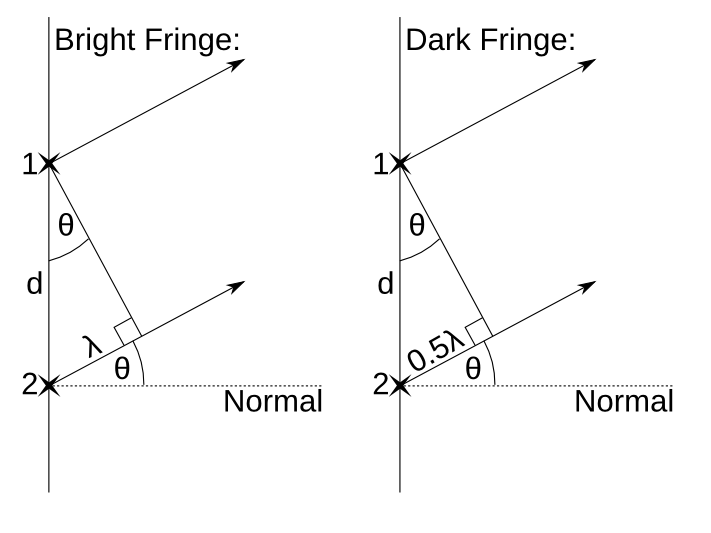
\includegraphics[scale = 0.5]{Diffraction.png}
    \caption{The path difference marked $\lambda$ may be any integer multiple of the wavelength i.e. $n\lambda$. By trigonometry we can also determine the length to be $d\sin\theta$}
    \label{fig:my_label}
\end{figure}

\section{Electricity}
Derive the resistance of two resistors in series. This starts by applying Ohm's law to each resistor individually, and use the fact that current remains constant through components in series.
\begin{gather*}
    V_T = V_1 + V_2 \\
    IR_T = IR_1 + IR_2 \\
    R_T = R_1 + R_2 \quad \qedsymbol
\end{gather*}

\newpage
We also need to do the same for two resistors in parallel, where we use the fact that will split between the two resistors such that $I_T = I_1 + I_2$ but voltage will be the same across each component. Once again we apply Ohm's law
\begin{gather*}
    I_T = I_1 + I_2 \\
    \cfrac{V}{R_T} = \cfrac{V}{R_1} + \cfrac{V}{R_2} \\
    \cfrac{1}{R_T} = \cfrac{1}{R_1} + \cfrac{1}{R_2} \quad \qedsymbol
\end{gather*}

\section{Magnetism}
Show that the force on a moving charge can be expressed as $F=qvB$. We start with the force on a current and use the principle of current as number of charges to pass a point per unit time. Finally velocity as length over time
\begin{align*}
    F=BIl \\
    F= B(\cfrac{q}{t})l \\
    F = q(\cfrac{l}{t}) B \\ 
    F = qvB
\end{align*}

\end{document}
